\documentclass[11pt,a4paper]{article} 
\usepackage{a4wide}
\linespread{1.25}
\usepackage{graphicx}
\usepackage{amssymb}
\usepackage{amsmath}
\usepackage{float}
\usepackage{graphicx}
\usepackage{natbib}
\usepackage{tikz}
\usepackage{caption}
\usepackage{subfig}
\usepackage[hmargin=3cm,vmargin=2cm]{geometry}
\usepackage{sidecap}
\usepackage{listings}
\usepackage{color}
\usepackage{multirow}
\thispagestyle{empty}
\usetikzlibrary{arrows}


\begin{document}

\pdfpageheight=7cm
\pdfpagewidth=12.5cm

\begin{figure}
\vspace{-1.9cm}

\hspace{-2.9cm}
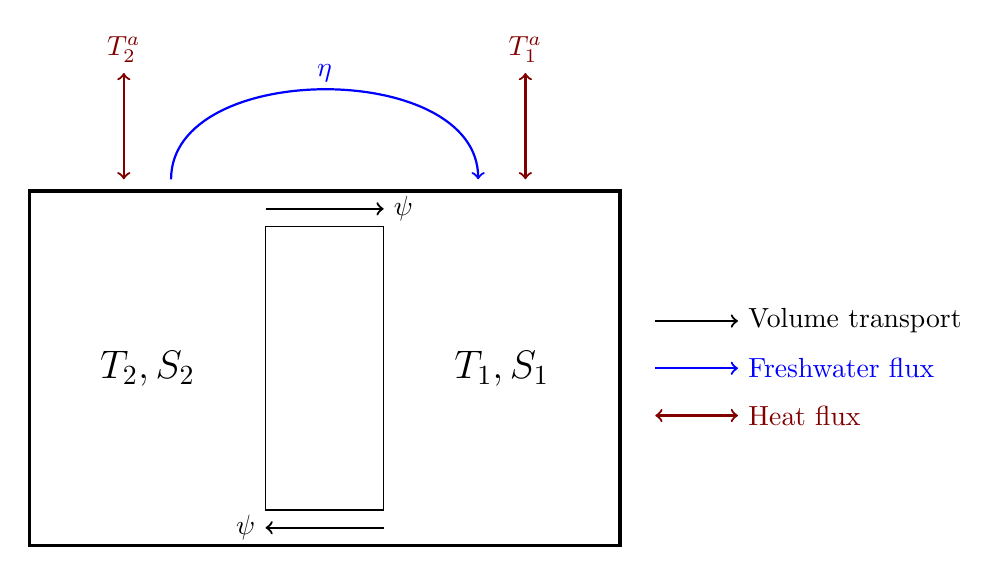
\begin{tikzpicture}[scale = 1.5]

\draw[black, very thick] (0, 0) -- (0, 3) -- (5, 3) -- (5, 0) -- cycle;
\draw[black] (2, 0.3) -- (2, 2.7) -- (3, 2.7) -- (3, 0.3) -- cycle;
\draw[->, thick] (2, 2.85) -- (3, 2.85) node[right] {$\psi$};
\draw[->, thick] (3, 0.15) -- (2, 0.15) node[left] {$\psi$};

\draw (1,1.5) node {{\Large $T_2, S_2$}};
\draw (4,1.5) node {{\Large $T_1, S_1$}};
  
\draw[<->, thick, red!50!black] (0.8, 3.1) -- (0.8, 4) node[above] {$T_2^{a}$};
\draw[<->, thick, red!50!black] (4.2, 3.1) -- (4.2, 4) node[above] {$T_1^{a}$};
\draw[blue, thick, ->] (1.2, 3.1) to [out=90,in=90] (3.8, 3.1);
\draw[blue] (2.5,4) node {$\eta$};

\draw [black, thick, ->] (5.3, 1.9) -- (6, 1.9) node[right] {Volume transport};
\draw [blue, thick, ->] (5.3, 1.5) -- (6, 1.5) node[right] {Freshwater flux};
\draw [red!50!black, thick, <->] (5.3, 1.1) -- (6, 1.1) node[right] {Heat flux};

\end{tikzpicture}
\end{figure}

$ $
\end{document}